%% abtex2-modelo-trabalho-academico.tex, v<VERSION> laurocesar
%% Copyright 2012-<COPYRIGHT_YEAR> by abnTeX2 group at http://www.abntex.net.br/ 

\documentclass[
	% -- opções da classe memoir --
	12pt,				% tamanho da fonte
	oneside,			% para impressão mudar para twoside para facilitar impressaõ de frente e verso 
	a4paper,			% tamanho do papel. 
	chapter=TITLE,
	sumario=tradicional,
	% -- opções do pacote babel --
	english,			% idioma adicional para hifenização
	brazil				% o último idioma é o principal do documento
]{abntex2}

% ----------------------------------------------------------
% IMPORTAÇÃO DE PACOTES
% ----------------------------------------------------------
\usepackage{helvet}
\renewcommand{\familydefault}{\sfdefault}			% Usa a fonte Arial			
\usepackage[T1]{fontenc}		% Selecao de codigos de fonte.
\usepackage[utf8]{inputenc}		% Codificacao do documento (conversão automática dos acentos)
\usepackage{indentfirst}		% Indenta $V_{in}$o primeiro parágrafo de cada seção.
\usepackage{color}				% Controle das cores
\usepackage{graphicx}			% Inclusão de gráficos
\usepackage{microtype} 			% para melhorias de justificação
\usepackage{hyperref}
\usepackage{times}

\usepackage{amsmath}
\usepackage{amsthm,amsfonts}

\usepackage{lipsum}				% para geração de dummy text
\usepackage{import}
\usepackage{blindtext}
\usepackage{soul}
\usepackage{lscape}

\graphicspath{ {./images/} }

% ---
% Pacotes de citações
% ---
\usepackage[alf]{abntex2cite}	% Citações padrão ABNT

% ----------------------------------------------------------
% CONFIGURAÇÕES DO PDF
% ----------------------------------------------------------

% alterando o aspecto da cor azul
\definecolor{blue}{RGB}{41,5,195}
\definecolor{black}{RGB}{0,0,0}

% informações do PDF
\makeatletter
\hypersetup{
     	%pagebackref=true,
		pdftitle={\@title}, 
		pdfauthor={\@author},
    	pdfsubject={\imprimirpreambulo},
	    pdfcreator={LaTeX with abnTeX2},
		pdfkeywords={abnt}{latex}{abntex}{abntex2}{trabalho acadêmico}, 
		colorlinks=true,       		% false: boxed links; true: colored links
    	linkcolor=black,          	% color of internal links
    	citecolor=black,        		% color of links to bibliography
    	filecolor=black,      		% color of file links
		urlcolor=black,
		bookmarksdepth=4
}
\makeatother

\setlrmarginsandblock{3cm}{2cm}{*}
\setulmarginsandblock{3cm}{2cm}{*}
\checkandfixthelayout

% --- 

% ----------------------------------------------------------
% FIGURAS E TABELAS
% ----------------------------------------------------------

% ---
% Posiciona figuras e tabelas no topo da página quando adicionadas sozinhas
% em um página em branco. Ver https://github.com/abntex/abntex2/issues/170
\makeatletter
\setlength{\@fptop}{5pt} % Set distance from top of page to first float
\makeatother
% ---

% ----------------------------------------------------------
% ESPAÇAMENTOS
% ----------------------------------------------------------

% O tamanho do parágrafo é dado por:
\setlength{\parindent}{1.25cm}

% % Controle do espaçamento entre um parágrafo e outro:
\setlength{\parskip}{0.2cm} 

\setlength{\ABNTEXcitacaorecuo}{4cm}

% Espaçamento entre headers e texto abaixo
\setlength\afterchapskip{0.2cm}
\setlength\aftersecskip{0.2cm} %espaçamento entre seção e texto
\setlength\aftersubsecskip{0.2cm} %espaçamento entre subseção e texto

% ----------------------------------------------------------
% CORREÇÕES DE ESTILO
% ----------------------------------------------------------

% Estilos das legendos
\captionnamefont{\ABNTEXfontereduzida}
\captiontitlefont{\ABNTEXfontereduzida}
\setlength{\belowcaptionskip}{1pt} % espaçamento depois do título das tabelas/figuras
\setlength{\abovecaptionskip}{1pt} % espaçamento antes da legenda de tabelas/figuras

% Estilos dos títulos

\renewcommand{\ABNTEXchapterfontsize}{\bfseries\normalsize}
\renewcommand{\ABNTEXsectionfontsize}{\itshape\normalsize}
\renewcommand{\ABNTEXsubsectionfontsize}{\normalfont\normalsize}
\renewcommand{\ABNTEXsubsubsectionfontsize}{\normalfont\normalsize}

\renewcommand{\chaptitlefont}{\normalfont\bfseries}
\setsecheadstyle{\normalfont\itshape}
\setsubsecheadstyle{\normalfont}
\setsubsubsecheadstyle{\normalfont}

\renewcommand{\ABNTEXchapterfont}{\bfseries}
\renewcommand{\ABNTEXchapterfontsize}{\normalsize}
\setboolean{ABNTEXupperchapter}{true}

% Estilos nos sumários
\renewcommand{\cftchapterfont}{\MakeUppercase}
\setboolean{ABNTEXupperchapter}{true}

\renewcommand{\cftsectionfont}{\normalfont}
\renewcommand{\cftsubsectionfont}{\normalfont}
\renewcommand{\cftsubsubsectionfont}{\normalfont}

% ----------------------------------------------------------
% COMPILA O ÍNDICE
% ----------------------------------------------------------
\makeindex

% ----------------------------------------------------------
% COMANDOS CUSTOMIZADOS
% ----------------------------------------------------------
\newcommand{\un}[1]{\;\text{#1}}
\newcommand{\logo}{\quad \Rightarrow \quad}
\newcommand{\codeword}[1]{\texttt{\textcolor{black}{#1}}}
\newcommand{\specialcell}[2][c]{%
  \begin{tabular}[#1]{@{}c@{}}#2\end{tabular}}

% ----------------------------------------------------------
% INÍCIO DO DOCUMENTO
% ----------------------------------------------------------
\begin{document}

%\selectlanguage{english}
\selectlanguage{brazil}

% Retira espaço extra obsoleto entre as frases.
\frenchspacing 

% ----------------------------------------------------------
% ELEMENTOS PRÉ-TEXTUAIS
% ----------------------------------------------------------
\begin{center}
\textbf{UNIVERSIDADE FEDERAL DE MINAS GERAIS\\
Escola de Engenharia \\
Curso de Bacharelado em Engenharia de Sistemas}

\vspace{4cm}

%\hspace{0.3\textwidth} \parbox{0.65\textwidth}
Cleyton Luan Nobre Assis 2021019815 \\
Maria Clara Oliveira Domingos Ruas 2021019572 \\
Raphael Henrique Braga Leivas 2020028101

\vspace{4cm}  

{ \textbf{Laboratório de Circuitos Eletrônicos e Projetos - Prática 2} }

\vfill
%\hspace{0.3\textwidth} 
{Belo Horizonte \\
2025 }
\end{center}

\newpage

% ---
% inserir o sumario
% ---
\pdfbookmark[0]{\contentsname}{toc}
\tableofcontents*
\cleardoublepage
% ---

% % ----------------------------------------------------------
% % ELEMENTOS TEXTUAIS
% % ----------------------------------------------------------
\textual

\pagestyle{simple}
	
\chapter{Objetivos}\label{cap:objetivos} 

\lipsum[1-2]

\chapter{Introdução}\label{cap:introdução} 

\lipsum[1-2]

\section{Experimento 2}

\subsection{Descrição}

Nesse experimento, vamos adicionar amplificadores operacionais para detectarem quando há sobrecorrente através do shunt.
Para isso, adicionamos subtrator U1 e o comparador U2, adicionando na saída do U2 um LED que acende quando a queda de tensão 
através do shunt passar de um dado limite, como mostra a \autoref{fig:circuito-exp2}.

\begin{figure}[h!]
	\caption{\label{fig:circuito-exp2}Circuito para o experimento 5.}
	\begin{center}
    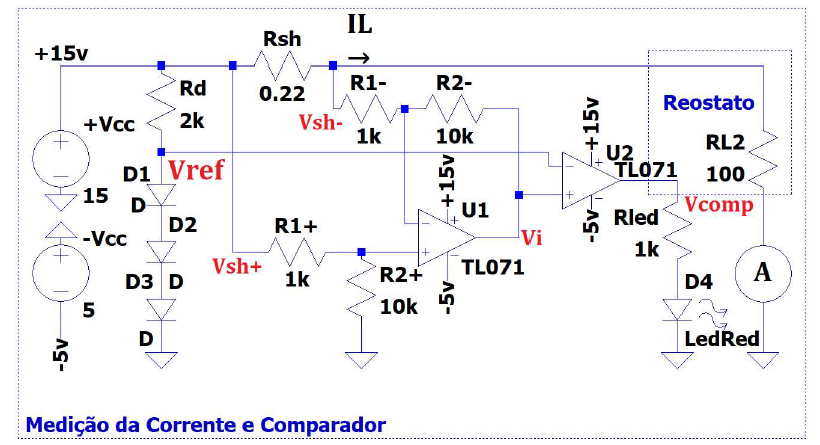
\includegraphics[width=0.8\textwidth,trim=1 1 1 1,clip]{images/circuito-exp2.png}
	\end{center}
	\legend{Fonte: elaboração própria.}
\end{figure}

\subsection{Resultados Obtidos}

Variando o reostato, vemos que o LED acende quando $R_L = 20 \Omega$. Nessa condições, 
temos as seguintes medições:

\begin{itemize}
	\item Corrente através da carga: $I_L = 0.97 \un{A}$
	\item Tensão através do shunt: $V_{sh} = 210.4 \un{mV}$
	\item Tensão na saída do U1 subtrator: $V_{oU1} = 2.1 \un{V}$
\end{itemize}

Assim, o ganho real do subtrator é

\[ G_{real} = \frac{V_{oU1}}{V_{sh}} = \frac{2.1 \un{V}}{210.4 \un{mV}} = 9.98 \]

A tensão $V_{ref}$ no instante que o LED acende foi medida em $V_{ref} = 2.06 \un{V}$.
Para que o LED acenda em exatamente $I_L = 1 \un{A}$, temos que o a tensão no shunt será de 
$V_{sh} = 220 \un{mV}$ nessa condição. Assim, precisamos que $R_1$ e $R_2$ do subtrator 
tenham um ganho de 

\[ G^* = \frac{R_2}{R_1} = \frac{2.06 \un{V}}{ 220 \un{mV}} = 9.36 \]

Assim, podemos usar $R_2 = 10 k\Omega$ e $R_1 = 1 k\Omega + 68 \Omega = 1068 \Omega$
para obter um ganho de exatamente 9.36 para que o LED acenda quando $I_L = 1 \un{A}$.

Dessa forma, para ter uma detecção de corrente ajustável, basta usar trimpots nos lugares 
de $R_2+$ e $R_2-$ no subtrator para ajustar o ganho do circuito. Reduzindo o trimpot, 
reduzimos o ganho do circuito e deixamos passar mais corrente que até que a queda de tensão 
através do shunt atinja o limite dos comparadores. Aumentando o trimpot, deixamos 
passar menos corrente.

Quando o LED está apagado, a saída medida do comparador é $V_{comp} = - 5.19 \un{V}$.
Com o LED aceso, temos a medição de $V_{comp} = 12.97 \un{V}$.
Essas faixas não são adequadas para usar como entrada de um circuito digital, uma vez que eles 
operam apenas na faixa de 0 a 5 V. Assim, podemos usar um diodo zener com $V_Z = 5.1 \un{V}$
para grampear a tensão positiva em 5 V, e um 1N4007 em série para proteger contra tensão negativa,
grampeando em 0V, como mostra a \autoref{fig:sim-exp2}. V1 simula a saída do comparador.

\begin{figure}[h!]
	\caption{\label{fig:sim-exp2}Circuito para ligar saída do comparador à lógica digital.}
	\begin{center}
    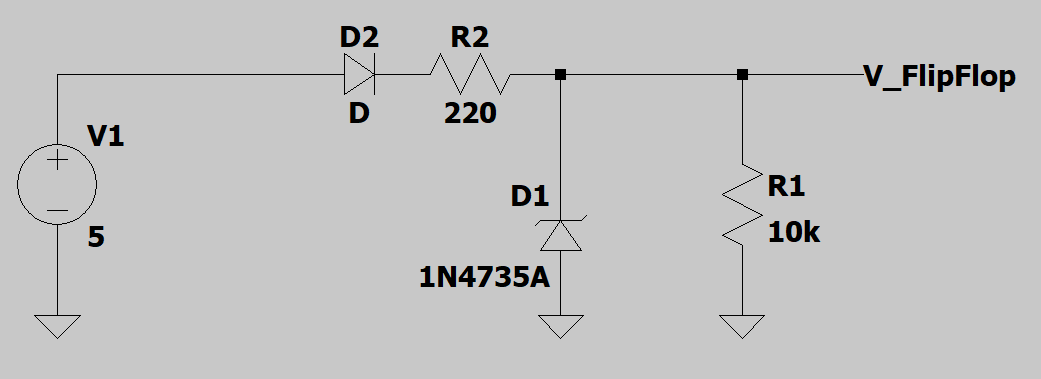
\includegraphics[width=0.75\textwidth,trim=1 1 1 1,clip]{images/sim-exp2.png}
	\end{center}
	\legend{Fonte: elaboração própria.}
\end{figure}

O funcionamento do circuito da \autoref{fig:sim-exp2} está simulado na 
\autoref{fig:result-sim-exp2}. Vemos que quando a saída do comparador (V1 no circuito) 
varia de -5V a 12V, a entrada do Flip Flop fica grampeada na faixa de 0 a 5V.


\begin{figure}[h!]
	\caption{\label{fig:result-sim-exp2}Funcionamento do circuito da proteção da lógica digital.}
	\begin{center}
    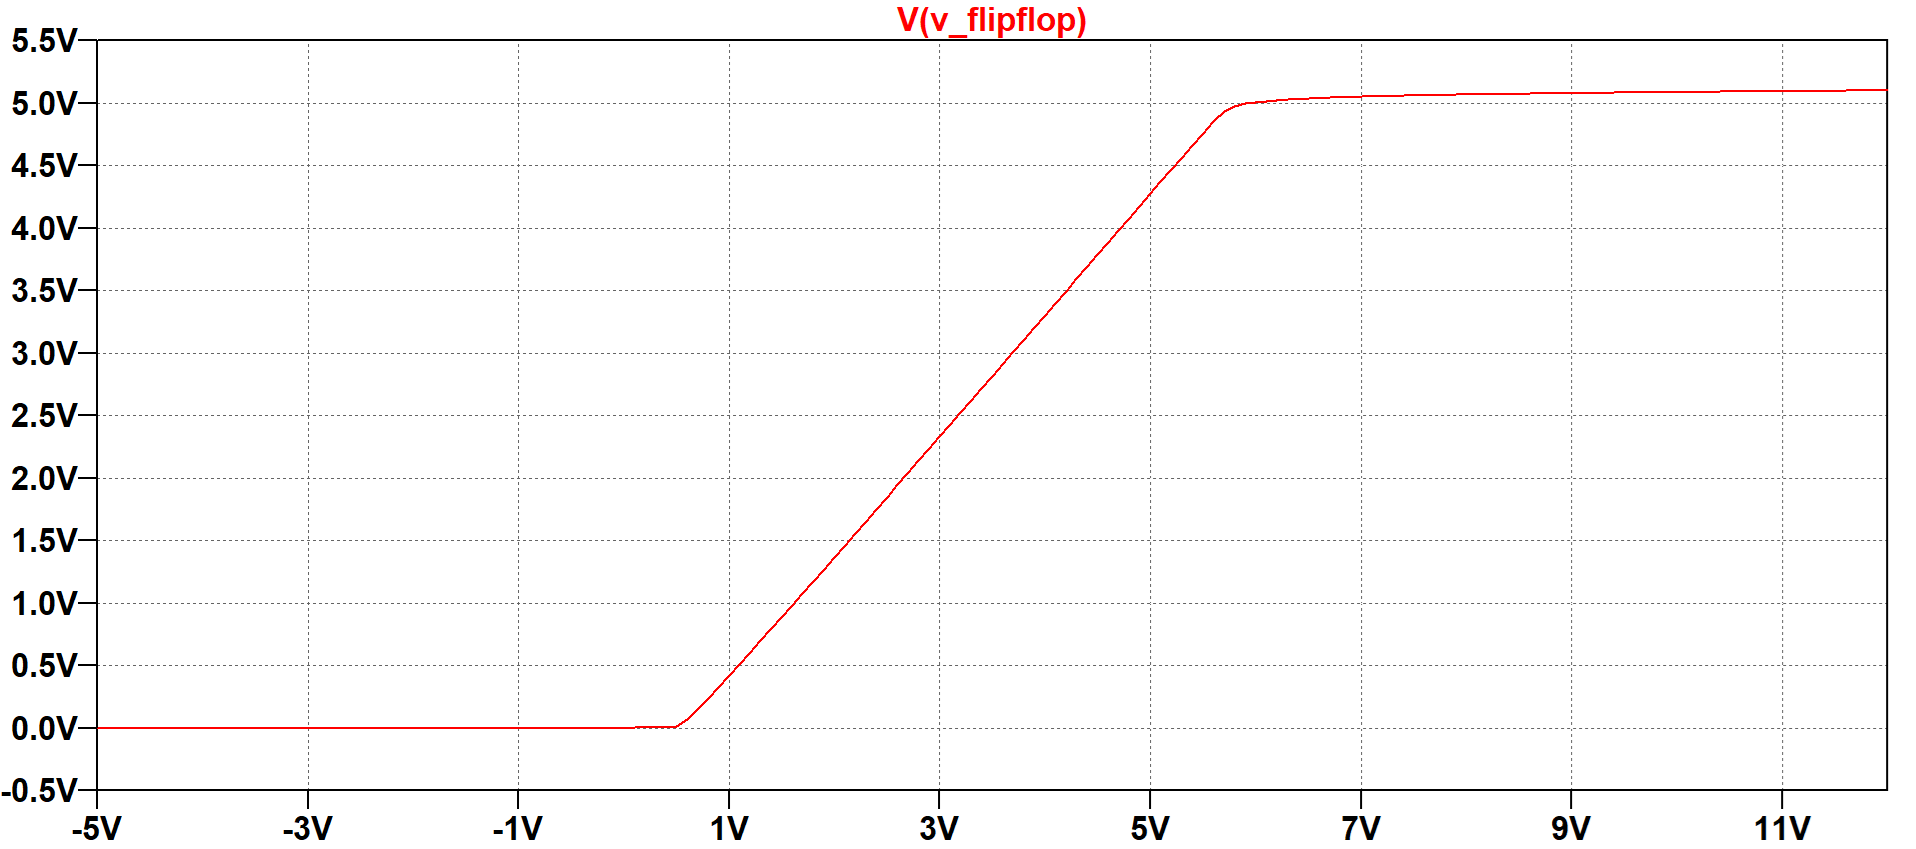
\includegraphics[width=\textwidth,trim=1 1 1 1,clip]{images/result-sim-exp2.png}
	\end{center}
	\legend{Fonte: elaboração própria.}
\end{figure}




\chapter{Conclusão}\label{cap:conclusao} 

Tendo em vista os objetivos da prática, foi possível verificar na prática os efeitos que o diodo zener, o BJT e 
o AmpOp possuem na regulagem na tensão de saída. 

Em particular, vimos como os efeitos indesejados da queda de tensão na carga - causada pelo aumento do dreno de corrente 
pela carga - pode ser atenuada pela presença do AmpOp com realimentação, de modo que o regulador de tensão a Zener e BJT,
apesar de simples, possui essa limitação.


\end{document}
